% ==============================================================================
% 第 29 章：带回溯的算法 (Chapter 29: Algorithms that Backtrack)
% ==============================================================================

\chapter{带回溯的算法}
\label{sec:ch29_backtracking}

解决问题的探索过程并不总是一帆风顺的笔直坦途。有时我们沿着某条途径不断向前推进，却因走错了岔路而陷入走投无路的僵局。此时最自然的解决策略便是：\term{回溯（backtrack）}到当初做出抉择的分岔路口，改选另一条尚未探索的分支重新尝试。诸多经典算法正是以这种机制运转的。本章深入剖析两个经典实例：第一节介绍图的路径遍历算法；第二节通过著名的国际象棋“$N$ 皇后谜题”展开综合性的回溯搜索项目设计。

\section{图的遍历}
\label{sec:29_1}

图（Graph）在真实世界与计算科学中无处不在。想象一个班级里的全体同学：写下每个人的名字，若两个人彼此相识，就在他们的名字之间画一条连接线。这样你就构建出了人生中的第一张\term{无向图（undirected graph）}。

现在考察图~\ref{fig:sample-graph}，它展现了一张小型\term{有向图（directed graph）}。该图由 7 个\term{节点（nodes}，即带圆圈的字母）和 9 条\term{有向边（edges}，即箭头）构成。这张图可以生动地代表某家公司的内部电子邮件交互网络：写下所有员工的邮箱地址，若员工 A 在一周内向员工 B 发送了邮件，就画一条从 A 指向 B 的单向箭头。

\begin{figure}[htbp]
  \centering
  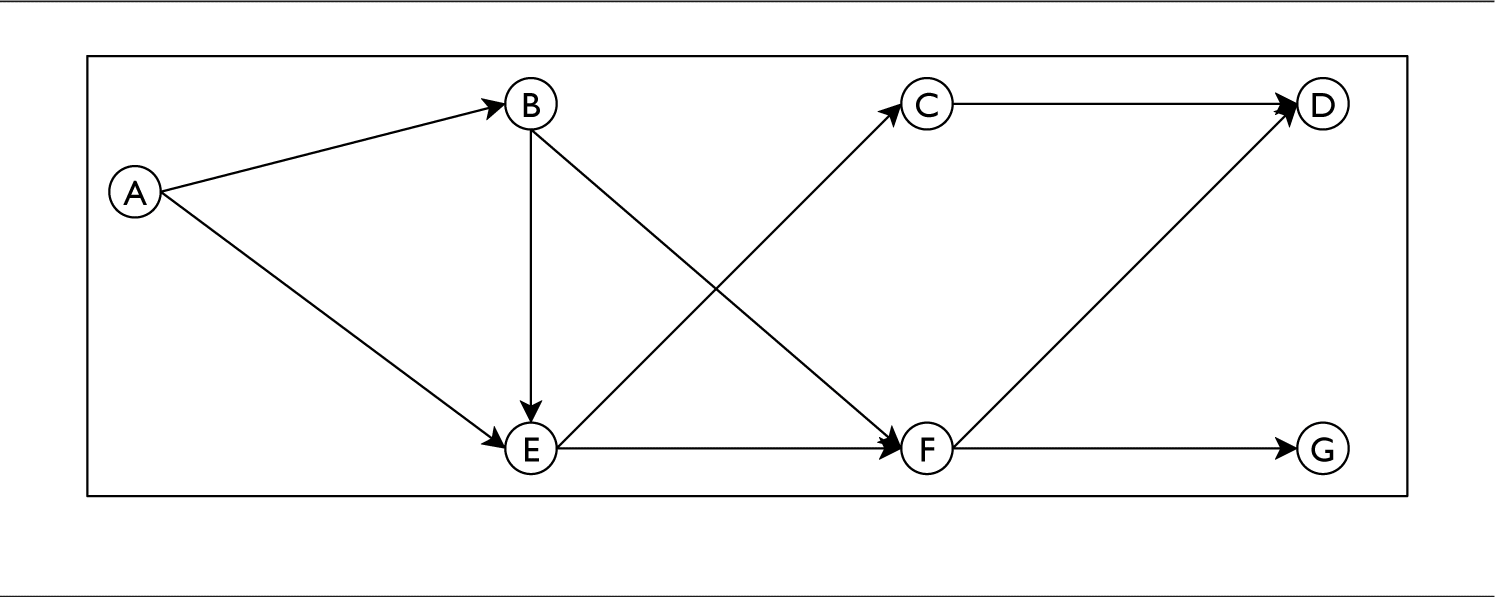
\includegraphics[width=0.75\textwidth]{images/00669.png}
  \caption{一个包含 7 个节点的小型有向图}
  \label{fig:sample-graph}
\end{figure}

形式化地，图由节点集合与连接节点的边集合构成。在有向图中，边代表单向关联；而在无向图中，边代表双向连通。在此背景下，如下是一个极具现实意义的典型问题：

\begin{notebox}[样例问题]
在某大型公司的内部邮件网络（有向图）中，设计一个算法为某员工规划向另一陌生员工递进引荐的联络路线。程序接收表示已建邮件通信的有向图以及两个邮箱节点，返回从起点连接到终点的一系列中间人邮箱序列。
\end{notebox}

数学家将这种从起点到终点的连通序列称为\term{路径（path）}。

图~\ref{fig:sample-graph} 将该问题具象化。例如，寻找从节点 \code{C} 到 \code{D} 的路径，该路径由起点 \code{C} 和终点 \code{D} 直接构成。而若要从 \code{E} 走到 \code{D}，则存在两条可选路径：
\begin{itemize}
  \item 从 \code{E} 经由 \code{F} 走向 \code{D}；
  \item 从 \code{E} 经由 \code{C} 走向 \code{D}。
\end{itemize}
有时两个节点之间可能根本不存在有效路径。例如在图~\ref{fig:sample-graph} 中，顺着箭头的方向无论如何也无法从 \code{C} 抵达 \code{G}。

如果将该有向图想象成一座大公园，你要从 \code{E} 走到 \code{G}：从 \code{E} 出发有两条岔路，一条通往 \code{C}，另一条通往 \code{F}。假定你先尝试第一条路走向 \code{C}，同时在脑海中记下“以后还可以尝试通往 \code{F} 的路线”。此时你面临一个全新问题：如何从 \code{C} 走到 \code{G}？这与原问题结构完全同构。然而从 \code{C} 出发无法到达 \code{G}，你陷入了死胡同。幸好，你记住了当初在 \code{E} 处还有另一条未走的选择，于是你\textbf{回溯}到 \code{E}，改走通往 \code{F} 的分支，最终顺利抵达目的地 \code{G}。

遵循设计配方，首先建立图的数据表示。图~\ref{fig:sample-graph} 可以表示为邻接表：
\begin{lstlisting}[language=BSL]
; Node 是 Symbol
; Graph 是 [List-of (list Node [List-of Node])]
; 或者 [List-of (cons Node [List-of Node])]

(define sample-graph
  '((A (B E))
    (B (E F))
    (C (D))
    (D ())
    (E (C F))
    (F (D G))
    (G ())))
\end{lstlisting}

\begin{exercise}{邻接表与 neighbors 函数设计}{471}\label{ex:471}
依据上述数据表示，设计函数 \code{neighbors}。它接收节点 \code{n} 与有向图 \code{g}，输出 \code{n} 在 \code{g} 中的直接后继邻居节点列表。
\end{exercise}

定义路径查找函数 \code{find-path} 的签名与目的说明：
\begin{lstlisting}[language=BSL]
; Node Node Graph -> [Maybe Path]
; 在有向图 G 中寻找一条从 origination 到 destination 的路径
; 若不存在连通路径，则返回 #false
(define (find-path origination destination G)
  #false)
\end{lstlisting}

回答生成型递归的四个设计问题：
\begin{enumerate}
  \item \textbf{平凡情形判断}：当起点与终点恰好是同一个节点时（\code{(symbol=? origination destination)}），问题平凡解决。
  \item \textbf{平凡解}：路径只包含该单一节点 \code{(list destination)}。
  \item \textbf{生成子问题}：若起点与终点不同，必须考察起点的所有直接邻居节点 \code{next = (neighbors origination G)}。遍历这些邻居并逐一递归探索从邻居到终点的路径。由于邻居是一个列表，我们提出一个辅助函数愿望清单：\code{find-path/list}。
  \item \textbf{合并子问题的解}：若在某个邻居节点上成功找到了通往终点的候选路径 \code{candidate}，只需将当前的 \code{origination} 节点拼装到该候选路径的最前端（\code{(cons origination candidate)}）即可构成完整路径；若所有邻居分支皆告失败，则返回 \code{\#false}。
\end{enumerate}

图~\ref{fig:find-path-code} 呈现了 \code{find-path} 与相互递归辅助函数 \code{find-path/list} 的完整定义。注意 \code{find-path/list} 对邻居列表采用结构型递归：对首个邻居调用 \code{find-path}，若返回的是非布尔路径则直接返回；否则，\textbf{回溯}探索剩余的邻居分支。

\begin{figure}[htbp]
  \centering
\begin{lstlisting}[language=BSL]
; Node Node Graph -> [Maybe Path]
; 寻找从 origination 到 destination 的路径，失败返回 #false
(define (find-path origination destination G)
  (cond
    [(symbol=? origination destination) (list destination)]
    [else (local ((define next (neighbors origination G))
                  (define candidate
                    (find-path/list next destination G)))
            (cond
              [(boolean? candidate) #false]
              [else (cons origination candidate)]))]))

; [List-of Node] Node Graph -> [Maybe Path]
; 从邻居列表 lo-Os 中寻找一条到达 D 的路径；若无路径则返回 #false
(define (find-path/list lo-Os D G)
  (cond
    [(empty? lo-Os) #false]
    [else (local ((define candidate
                    (find-path (first lo-Os) D G)))
            (cond
              [(boolean? candidate)
               (find-path/list (rest lo-Os) D G)]
              [else candidate]))]))
\end{lstlisting}
  \caption{图中的路径查找与回溯算法}
  \label{fig:find-path-code}
\end{figure}

\begin{exercise}{测试 find-path 与全节点连通测试}{472}\label{ex:472}
测试 \code{find-path}：使用它寻找 \code{'A} 到 \code{'G} 的路径。它找到的是哪一条路径？为什么？
设计函数 \code{test-on-all-nodes}，接收图 \code{g}，判定是否在任意节点对之间均能正确返回路径或 \code{\#false}。
\end{exercise}

现在考察算法的停机性。在无环图（DAG）中，由于节点总数有限且无环路折返，\code{find-path} 必然停机。然而，若图中存在\term{环路（cycle）}，情况便急转直下。考察图~\ref{fig:cyclic-graph}：相比图~\ref{fig:sample-graph}，它仅增加了一条从 \code{C} 指向 \code{B} 的反向边。

\begin{figure}[htbp]
  \centering
  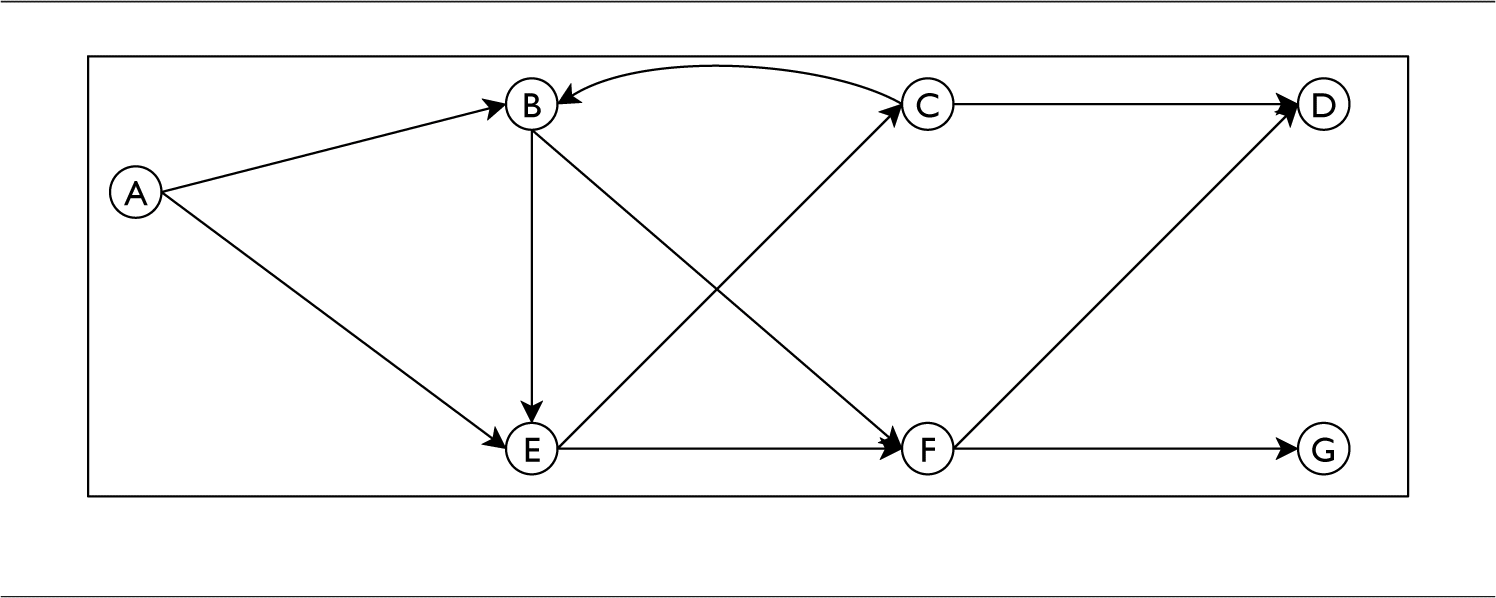
\includegraphics[width=0.75\textwidth]{images/00675.png}
  \caption{包含环路的有向图}
  \label{fig:cyclic-graph}
\end{figure}

如果在此有环图上执行 \code{(find-path 'B 'D cyclic-graph)}，算法将沿着 $B \to E \to C \to B$ 不断循环转圈，陷入死循环！
手工推导表明：在 7 步相互递归调用后，求值环境再次面临完全相同的表达式 \code{(find-path 'B 'D cyclic-graph)}。由于缺乏已访问节点的记忆机制，函数在此类有环图上无法停机。在第 VI 部分中，我们将借助“累加器”记录访问历史来彻底攻克这一难题。

\begin{exercise}{环路图上的行为测试}{473}\label{ex:473}
在图~\ref{fig:cyclic-graph} 所示的有环图上测试 \code{find-path 'B 'C cyclic-graph}，观察 DrRacket 的执行表现。
\end{exercise}

\begin{exercise}{单函数重构 find-path}{474}\label{ex:474}
使用 \code{local} 表达式将 \code{find-path} 与 \code{find-path/list} 整合重构为一个单一的顶级函数。
\end{exercise}

\begin{exercise}{使用 ormap 重构 find-path/list}{475}\label{ex:475}
能否利用列表抽象函数（如标准库中的高阶函数）来消除显式的结构型递归？探索 Racket 的 \code{ormap} 与 ISL+ 的不同之处，评估其在此处的适用性。
\end{exercise}

\begin{exercise}{有限状态自动机字符匹配 fsm-match?}{476}\label{ex:476}
设计函数 \code{fsm-match?}。它接收有限状态自动机（FSM）的数据表示与字符串，判断该字符串是否能驱动该自动机从初始状态转移并最终停留在接受状态。
提示：在 \code{local} 中定义辅助函数，将计算状态表示为当前状态与剩余字符列表的二元对。
\end{exercise}

\begin{figure}[htbp]
  \centering
\begin{lstlisting}[language=BSL]
; [List-of X] -> [List-of [List-of X]]
; 生成列表 w 中所有元素的全排列列表
(define (arrangements w)
  (cond
    [(empty? w) '(())]
    [else
     (foldr (lambda (item others)
              (local ((define without-item
                        (arrangements (remove item w)))
                      (define add-item-to-front
                        (map (lambda (a) (cons item a))
                             without-item)))
                (append add-item-to-front others)))
            '()
            w)]))
\end{lstlisting}
  \caption{基于生成型递归与列表抽象的全排列算法}
  \label{fig:arrangements-code}
\end{figure}

\begin{exercise}{基于生成型递归的排列全排列 arrangements}{477}\label{ex:477}
图~\ref{fig:arrangements-code} 展示了通过生成型递归与 \code{foldr}、\code{map} 组合实现的全排列生成函数 \code{arrangements}。
阐明其算法设计逻辑，回答生成型递归的全部核心问题，并为其撰写终止性论证。该实现生成的排列列表与第 12.4 节中的顺序是否完全一致？
\end{exercise}

\section{综合项目：N 皇后谜题}
\label{sec:29_2}

国际象棋中的\term{$N$ 皇后谜题（$n$ queens puzzle）}是展示回溯算法魅力的极佳典范。一个标准国际象棋棋盘由 $n \times n$ 个方格组成。皇后可以沿水平、垂直或对角线方向移动任意距离（如图~\ref{fig:queen-threat} 所示）。若某方格处于皇后的行进路线上，称该方格受到该皇后的\term{攻击威胁（threatened）}。

\begin{figure}[htbp]
  \centering
  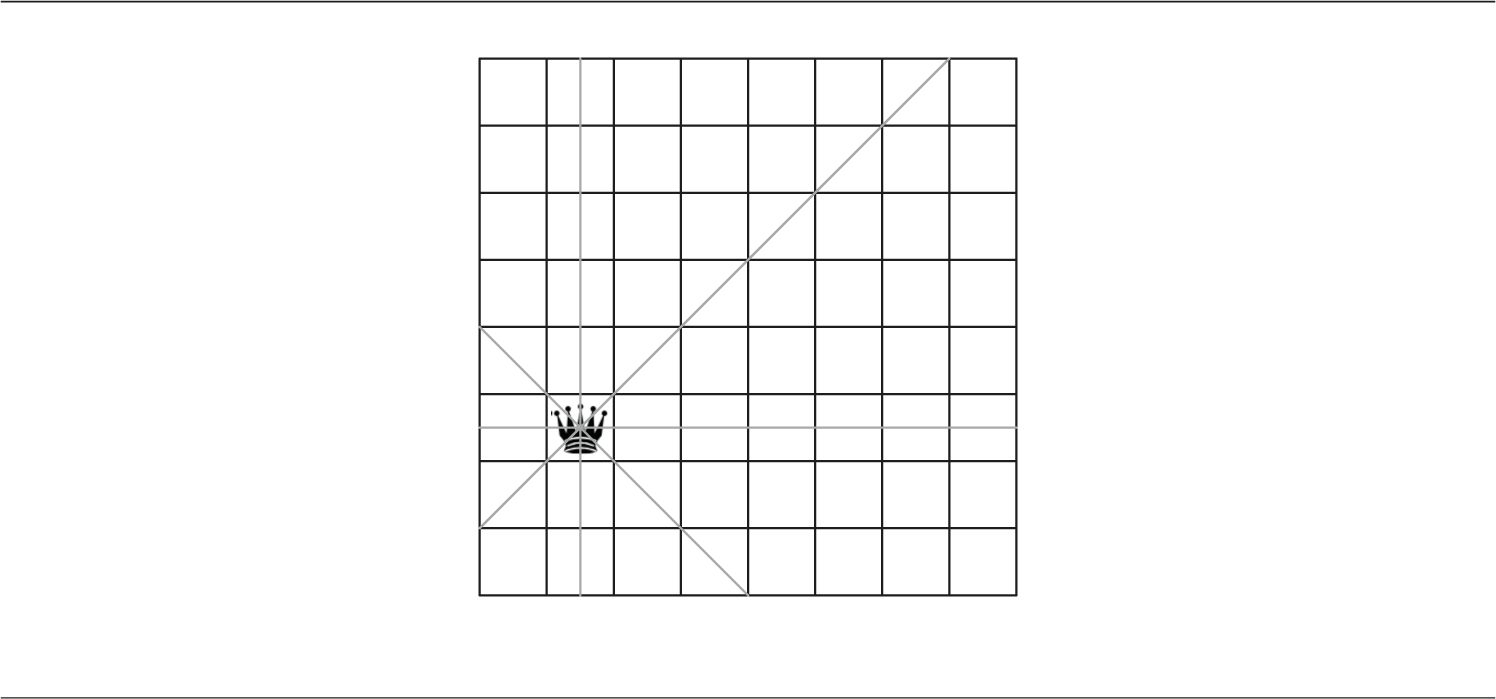
\includegraphics[width=0.65\textwidth]{images/00678.jpeg}
  \caption{棋盘上的单个皇后及其辐射威胁范围}
  \label{fig:queen-threat}
\end{figure}

经典 8 皇后问题要求在 $8 \times 8$ 棋盘上放置 8 个皇后，使得彼此互不受攻击。计算机科学家将其推广为任意规模的 $n$ 皇后谜题。显然，当 $n = 2$ 或 $n = 3$ 时，谜题无解（如图~\ref{fig:queens-3x3} 所示，放置两个互不攻击的皇后后，棋盘已无任何安全空格可供第三个皇后安放）。图~\ref{fig:queens-solutions} 给出了 $n=4$ 与 $n=5$ 的可行解。

\begin{figure}[htbp]
  \centering
  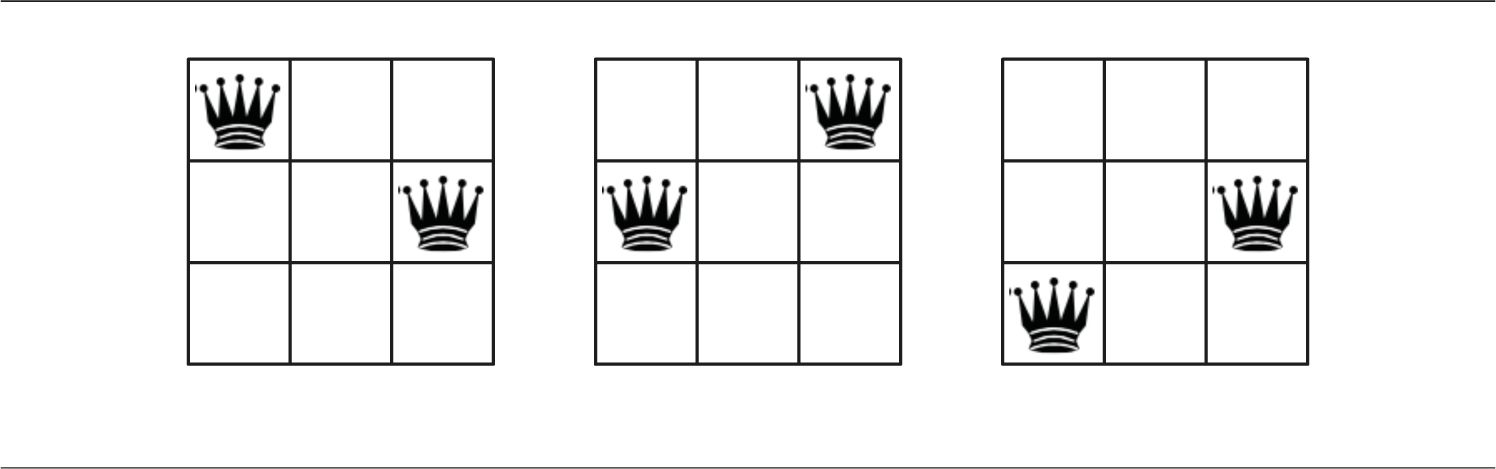
\includegraphics[width=0.75\textwidth]{images/00679.jpeg}
  \caption{$3 \times 3$ 棋盘上放置两个皇后的所有尝试均导致剩余方格全受威胁}
  \label{fig:queens-3x3}
\end{figure}

\begin{figure}[htbp]
  \centering
  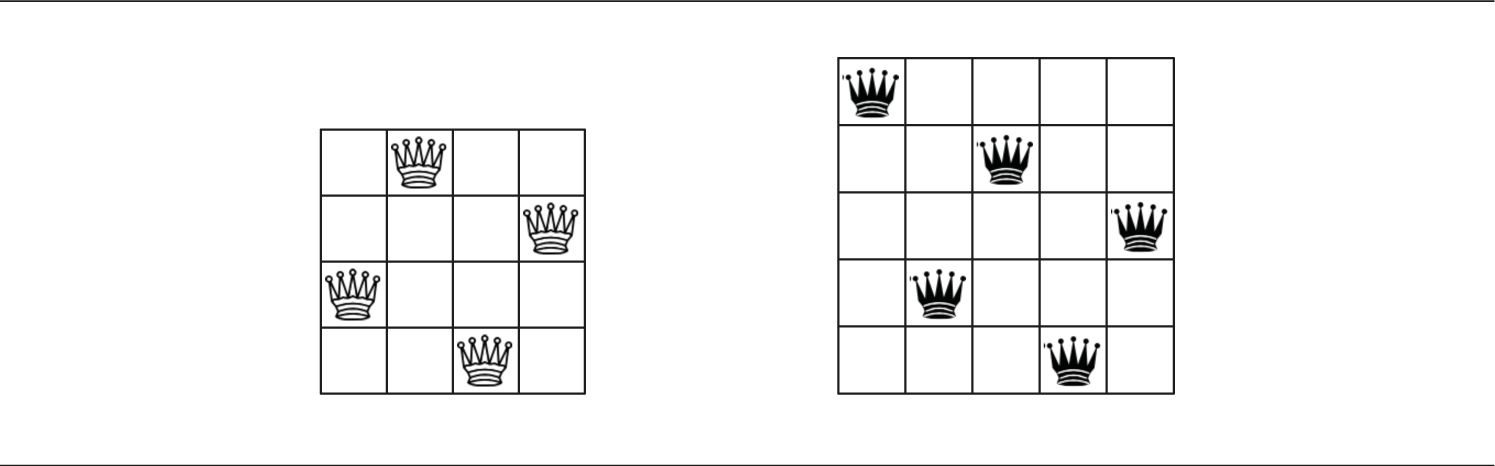
\includegraphics[width=0.85\textwidth]{images/00680.jpeg}
  \caption{$4 \times 4$ 与 $5 \times 5$ 棋盘的 $N$ 皇后合法解}
  \label{fig:queens-solutions}
\end{figure}

求解 $N$ 皇后问题的回溯思维如下：
\begin{enumerate}
  \item 一次放置一个皇后。放置后，标记其辐射的所有行、列与对角线为不可用；
  \item 对于下一个皇后，仅考虑尚未受到威胁的安全空位；
  \item 记录当前步骤的所有可选安全格；
  \item 若在某一阶段需要放置皇后却无任何安全空格可用，则说明先前的选择有误，立即\textbf{回溯}到上一步，改选上一步的下一个备选空格继续尝试。
\end{enumerate}

棋盘位置的数据表示：
\begin{lstlisting}[language=BSL]
(define QUEENS 8)

; QP 是结构体：(make-posn CI CI)
; CI 是区间 [0, QUEENS) 内的自然数
; 解释：(make-posn r c) 表示位于第 r 行第 c 列的方格
\end{lstlisting}

\begin{exercise}{威胁判断函数 threatening?}{479}\label{ex:479}
设计函数 \code{threatening?}。它接收两个 \code{QP} 位置，判定放置在两处的皇后是否会相互威胁。
数学洞见：
\begin{itemize}
  \item 水平威胁：行坐标相等（$r_1 = r_2$）；
  \item 垂直威胁：列坐标相等（$c_1 = c_2$）；
  \item 45 度对角线威胁：坐标和相等（$r_1 + c_1 = r_2 + c_2$）；
  \item 135 度对角线威胁：坐标差绝对值相等（$|r_1 - c_1| = |r_2 - c_2|$）。
\end{itemize}
\end{exercise}

\begin{exercise}{棋盘与皇后的图形化绘制 render-queens}{480}\label{ex:480}
设计函数 \code{render-queens}。接收自然数 $n$、皇后位置列表 \code{[List-of QP]} 以及棋子图像，绘制带有皇后的 $n \times n$ 棋盘。
\end{exercise}

算法主体 \code{n-queens} 的顶层定义如图~\ref{fig:n-queens-code} 所示。它将任务委托给辅助回溯函数 \code{place-queens}。

\begin{figure}[htbp]
  \centering
\begin{lstlisting}[language=BSL]
; N -> [Maybe [List-of QP]]
; 求解 n 皇后问题，成功返回皇后坐标列表，无解返回 #false

(define (n-queens n)
  (place-queens (board0 n) n))
\end{lstlisting}
  \caption{$N$ 皇后主求解函数}
  \label{fig:n-queens-code}
\end{figure}

\begin{exercise}{解的性质验证与集合等价谓词}{481}\label{ex:481}
设计高阶谓词 \code{n-queens-solution?}：接收 $n$，生成用于检验候选位置列表是否为有效 $n$ 皇后解的谓词（长度为 $n$ 且任意两两互不威胁）。
设计集合等价函数 \code{set=?}，判定两个列表在忽略元素次序的前提下是否包含完全相同的元素。
\end{exercise}

\begin{exercise}{核心放置算法 place-queens}{482}\label{ex:482}
依据回溯策略设计 \code{place-queens}：
\begin{lstlisting}[language=BSL]
; Board N -> [Maybe [List-of QP]]
; 在已有棋盘 a-board 上放置剩余的 n 个皇后；若无解返回 #false
(define (place-queens a-board n)
  #false)
\end{lstlisting}
假设针对棋盘抽象数据类型已拥有如下愿望清单函数：
\begin{itemize}
  \item \code{board0}：创建初始的空棋盘；
  \item \code{add-queen}：在棋盘的指定位置放置皇后并更新受威胁状态；
  \item \code{find-open-spots}：返回当前棋盘上所有依然安全的开阔空位列表。
\end{itemize}
\end{exercise}

\begin{exercise}{棋盘的三种数据表示与数据抽象}{483}\label{ex:483}
为 \code{Board} 设计具体的数据表示并实现练习~\ref{ex:482} 中的愿望清单函数。考虑以下三种不同建模思路：
\begin{enumerate}
  \item 棋盘表示为当前所有\textbf{仍可放置皇后的安全方格}列表；
  \item 棋盘表示为\textbf{已放置的所有皇后位置}列表；
  \item 棋盘表示为一个包含 $n \times n$ 个方格结构体的网格列表，每个格子记录自身坐标及是否受威胁的状态。
\end{enumerate}
体会数据抽象的威力：只要底层接口保持一致，算法核心代码无需做任何修改即可无缝运行！
\end{exercise}
